\documentclass[xcolor=pdftex,table,10pt]{beamer}

\mode<presentation> {
  \usetheme{Madrid}
  \usecolortheme{seahorse}
  \usecolortheme{rose}
}

\AtBeginSection[]
{
  \begin{frame}<beamer>
    \frametitle{Outline}
    \tableofcontents[currentsection,hideothersubsections]
  \end{frame}
}

\AtBeginSubsection[]
{
  \begin{frame}<beamer>
    \frametitle{Outline}
    \tableofcontents[currentsection,currentsubsection]
  \end{frame}
}

%change bottom line
\setbeamertemplate{footline}
{
  \leavevmode%
  \hbox{%
  \begin{beamercolorbox}[wd=.23\paperwidth,ht=2.25ex,dp=1ex,center]{author in head/foot}%
    \usebeamerfont{author in head/foot}\insertshortauthor
  \end{beamercolorbox}%
  \begin{beamercolorbox}[wd=.54\paperwidth,ht=2.25ex,dp=1ex,center]{title in head/foot}%
    \usebeamerfont{title in head/foot}\insertshorttitle
  \end{beamercolorbox}%
  \begin{beamercolorbox}[wd=.23\paperwidth,ht=2.25ex,dp=1ex,right]{date in head/foot}%
    \usebeamerfont{date in head/foot}\insertshortdate{}\hspace*{2em}
    \insertframenumber{} / \inserttotalframenumber\hspace*{2ex} 
  \end{beamercolorbox}}%
  \vskip0pt%
}

\usepackage[english]{babel}
\usepackage[latin1]{inputenc}
\usepackage{times}
%\usepackage[T1]{fontenc}
%\usepackage{color}
%\usepackage[x11names, rgb]{xcolor}
\usepackage{listings}
\usepackage{colortbl}
%\usepackage{dot2texi}
\usepackage{tikz}
\usepackage{verbatim}
%\usepackage{pgfplots}
%\usetikzlibrary{arrows,shapes,backgrounds,snakes}
\usetikzlibrary{arrows}
%\usefonttheme{professionalfonts}
\usefonttheme[onlymath]{serif}

\title{A Parallel Multigrid Solver for Beam Dynamics}
\author{Yves Ineichen (ETH Zurich)}
\institute{\textbf{Master Thesis} \\ Supervisor: Andreas Adelmann (PSI), Peter Arbenz (ETH)}
\date{10th April 2008}
%\logo{
\includegraphics[width=3cm]{psilogo}}
\titlegraphic{
	\begin{columns}
		\begin{column}{3cm}
			
\includegraphics[width=3cm]{psilogo} \\
		\end{column}
		\begin{column}{2cm}
			\includegraphics[width=2cm]{ethlogo} \\
		\end{column}
	\end{columns}
}

\begin{document}

% For every picture that defines or uses external nodes, you'll have to
% apply the 'remember picture' style. To avoid some typing, we'll apply
% the style to all pictures.
\tikzstyle{every picture}+=[remember picture]

% By default all math in TikZ nodes are set in inline mode. Change this to
% displaystyle so that we don't get small fractions.
\everymath{\displaystyle}

	\lstset{language=C++, basicstyle=\small}

	\begin{frame}
		\titlepage
	\end{frame}
	
	\begin{frame}
	  \frametitle{Outline}
	  \tableofcontents
	\end{frame}

	\section{Motivation}

	\begin{frame}
		\frametitle{Motivation}
		\framesubtitle{OPAL: state of the art}

		At the moment OPAL space-charge forces are calculated using:

		\begin{itemize}
			\item (parallel) FFT based direct solver for the Poisson equation
			\item convolution with an improved Green's function
			\item open boundaries are assumed
		\end{itemize}

		\pause
		\vspace{0.7cm}

		To improve the simulation for users:
		
		\vspace{0.3cm}

		\begin{alertblock}{Goals}
		\begin{itemize}
			\item try to speed-up computation of electrostatic fields
			\item handle complicated beam pipe boundary conditions
		\end{itemize}
		\end{alertblock}

	\end{frame}
	
	\begin{frame}

		\frametitle{Motivation}
		\framesubtitle{problem formulation}

		\begin{block}{Problem Statement}
		Solve the electrostatic Poisson PDE on an anisotropic (particles moving near lightspeed) rectangular grid in nonrectangular domains (motivated by the beam pipe geometry).
		\end{block}

		\pause
		\vspace{0.9cm}

		The problem can be broken down in sub-steps

		\begin{enumerate}
			\item implement and optimize a ML preconditioned solver
			\item incorporate this solver into OPAL
			\item handle the irregular boundary points
			\item investigate and implement ways to enable OPAL to use exact beam pipe geometries
		\end{enumerate}

	\end{frame}

    %CONTENT: explain mg, sa (short), benefits (AND reusing old solution as approx),
    \section{Multigrid Theory}

    	\begin{frame}
		\frametitle{Multigrid Theory (1/2)}
		\framesubtitle{Motivation}

		\begin{block}{Important Observations}
			\begin{itemize}
				\item Some classical iterative methods (i.e. Gauss Seidel) have a smoothing effect on the error of any approximation for discrete elliptic problems.
				\vspace{0.2cm}
				\item A smooth error can be well approximated on a coarse grid. This coarse grid has considerably fewer grid points and is therefore cheaper to solve.
			\end{itemize}
		\end{block}

		\pause
		\vspace{0.4cm}

		From this two observations a Two-Grid can be deduced:

		\begin{enumerate}
			\item apply smoother
			\item restrict to a grid with considerably fewer grid points (coarse)
			\item solve
			\item interpolate back to the fine grid
			\item compute a new approximation
		\end{enumerate}

	\end{frame}
    	
	\begin{frame}
		\frametitle{Multigrid Theory (2/2)}
		\framesubtitle{The Two-Grid: Smoothed Coarse Grid Correction}

		The discretized system is solved by a Two-Grid:

		\[
			A\mathbf{x} = \mathbf{b}
		\]
		\[
			e_h^m = x_h - x_h^m\text{, } r_h^m = b_h - A_hx_h^m
		\]
		\[
			r_h^m = A_h e_h^m
		\]

		\vspace{0.1cm}

		\begin{center}
		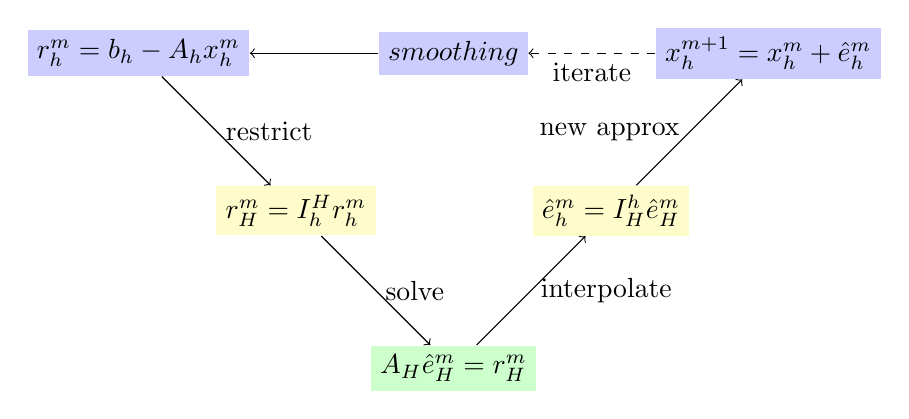
\begin{tikzpicture}[scale=1,transform shape,node distance=2cm]	
            		\node[fill=blue!20] (res)
            		{$ r_h^m = b_h - A_h x_h^m $};
			\node[right of=res] (dummy6) {};
            		\node[fill=blue!20, right of=dummy6] (smooth)
            		{$ smoothing $};
			\node[below of=res] (dummy1) {};
            		\node[fill=yellow!20, right of=dummy1] (restrict)
            		{$ r_H^m = I_h^H r_h^m$};
			\node[below of=restrict] (dummy2) {};
            		\node[fill=green!20, right of=dummy2] (solve)
            		{$ A_H \hat{e}_H^m = r_H^m $};
			\node[right of=solve] (dummy3) {};
            		\node[fill=yellow!20, above of=dummy3] (interpolate)
            		{$ \hat{e}_h^m = I_H^h \hat{e}_H^m $};
			\node[right of=interpolate] (dummy4) {};
            		\node[fill=blue!20, above of=dummy4] (newapprox)
			{$ x_h^{m+1} = x_h^m + \hat{e}_h^m $};

        		\path[->] (res) edge node[right] {restrict} (restrict);
        		\path[->] (restrict) edge node[right] {solve} (solve);
        		\path[->] (solve) edge node[right] {interpolate} (interpolate);
        		\path[->] (interpolate) edge node[left] {new approx} (newapprox);
        		\path[->] (smooth) edge (res);
        		\path[->,dashed] (newapprox) edge node[below] {iterate} (smooth);
		\end{tikzpicture}
		\end{center}

	\end{frame}

	\begin{frame}
		\frametitle{Grid Operators}

		\begin{columns}
		\begin{column}{4.5cm}
		\textbf{restriction} \\
		\vspace{0.4cm}
		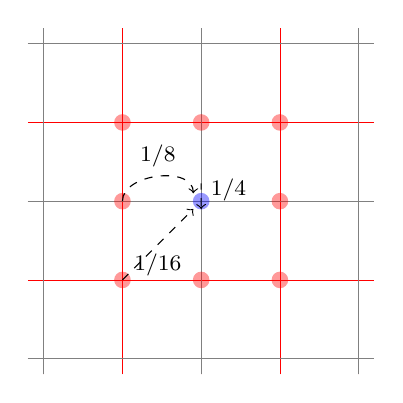
\begin{tikzpicture}[scale=1.0,transform shape,node distance=1cm]	
			\draw[very thin,color=red,step=1cm] (-0.2,-0.2) grid (4.2,4.2);
			\draw[very thin,color=gray,step=2cm] (-0.2,-0.2) grid (4.2,4.2);
			
			%\draw[very thin,color=gray,step=2cm] (5,-0.2) grid (9.2,4.2);
    
			\fill[color=blue,opacity=0.4] (2.0,2.0) circle (3pt);
			\fill[color=red,opacity=0.4] (1.0,2.0) circle (3pt);
			\fill[color=red,opacity=0.4] (1.0,1.0) circle (3pt);
			\fill[color=red,opacity=0.4] (2.0,1.0) circle (3pt);
			\fill[color=red,opacity=0.4] (3.0,2.0) circle (3pt);
			\fill[color=red,opacity=0.4] (2.0,3.0) circle (3pt);
			\fill[color=red,opacity=0.4] (3.0,3.0) circle (3pt);
			\fill[color=red,opacity=0.4] (1.0,3.0) circle (3pt);
			\fill[color=red,opacity=0.4] (3.0,1.0) circle (3pt);
			
    			\path[style=dashed, ->] (1.0,2.0) edge [out=90, in=90] node[above] {\footnotesize{$1/8$}} (1.9,2.1);
    			\path[style=dashed, ->] (1.0,1.0) edge node[below] {\footnotesize{$1/16$}} (1.9,1.9);
    			\path[style=dashed, ->] (2.0,2.2) edge [out=90, in=91] node[right] {\footnotesize{$1/4$}} (2.0,1.9);

		\end{tikzpicture}
		\end{column}

		\begin{column}{4.5cm}
		\textbf{bilinear interpolation} \\
		\vspace{0.4cm}
		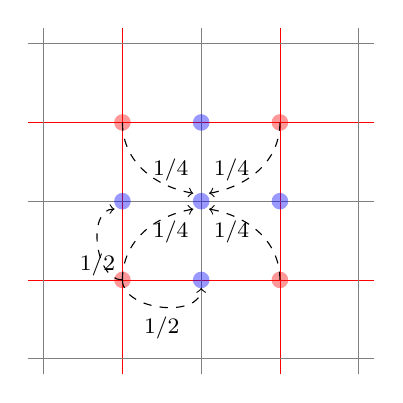
\begin{tikzpicture}[scale=1.0 ,transform shape,node distance=1cm]	
			\draw[very thin,color=red,step=1cm] (-0.2,-0.2) grid (4.2,4.2);
			\draw[very thin,color=gray,step=2cm] (-0.2,-0.2) grid (4.2,4.2);
			
			%\draw[very thin,color=gray,step=2cm] (5,-0.2) grid (9.2,4.2);
    
			\fill[color=blue,opacity=0.4] (2.0,2.0) circle (3pt);
			\fill[color=blue,opacity=0.4] (1.0,2.0) circle (3pt);
			\fill[color=red,opacity=0.4] (1.0,1.0) circle (3pt);
			\fill[color=blue,opacity=0.4] (2.0,1.0) circle (3pt);
			\fill[color=blue,opacity=0.4] (3.0,2.0) circle (3pt);
			\fill[color=blue,opacity=0.4] (2.0,3.0) circle (3pt);
			\fill[color=red,opacity=0.4] (3.0,3.0) circle (3pt);
			\fill[color=red,opacity=0.4] (1.0,3.0) circle (3pt);
			\fill[color=red,opacity=0.4] (3.0,1.0) circle (3pt);
			
    			
			\path[style=dashed, ->] (3.0,3.0) edge [out=-90, in=10] node[left] {\footnotesize{$1/4$}} (2.1,2.1);
    			\path[style=dashed, ->] (1.0,3.0) edge [out=-90, in=170] node[right] {\footnotesize{$1/4$}} (1.9,2.1);
    			\path[style=dashed, ->] (3.0,1.0) edge [out=90, in=-10] node[left] {\footnotesize{$1/4$}} (2.1,1.9);
    			\path[style=dashed, ->] (1.0,1.0) edge [out=90, in=-170] node[right] {\footnotesize{$1/4$}} (1.9,1.9);

    			\path[style=dashed, ->] (1.0,1.0) edge [out=-90, in=-90] node[below] {\footnotesize{$1/2$}} (2.0,0.9);
    			\path[style=dashed, ->] (1.0,1.0) edge [out=180, in=180] node[below] {\footnotesize{$1/2$}} (0.9,1.9);
		\end{tikzpicture}
		\end{column}
		\end{columns}

	\end{frame}
	

	\begin{frame}
		\frametitle{Multigrid}
		\framesubtitle{from Two-Grid to Multigrid}

		%v -> V / W (etc)
		\begin{center}
		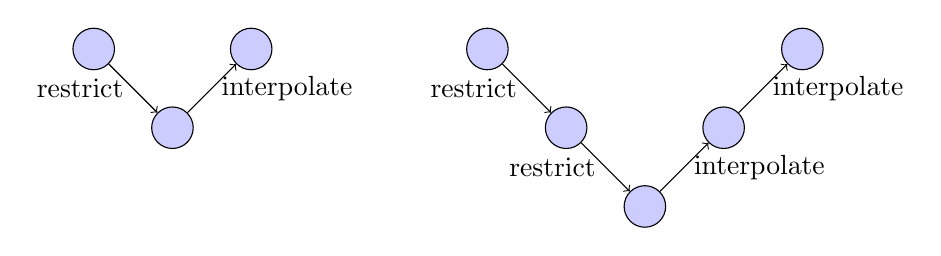
\begin{tikzpicture}[scale=1,transform shape,node distance=1cm]	
			\tikzstyle{circ} = [circle, draw, thin, fill=blue!20, minimum height=1.5em]

			%v
			\node[circ] (v1) {};
			\node[right of=v1] (dummy1) {};
			\node[circ,below of=dummy1] (v2) {};
			\node[circ,right of=dummy1] (v3) {};
        		\path[->] (v1) edge node[left] {restrict} (v2);
        		\path[->] (v2) edge node[right] {interpolate} (v3);
			
			%V
			\node[right of=v3] (DD) {};
			\node[right of=DD] (D) {};
			\node[circ,right of=D] (V1) {};
			\node[right of=V1] (Dummy1) {};
			\node[circ,below of=Dummy1] (V2) {};
			\node[right of=V2] (Dummy2) {};
			\node[circ,below of=Dummy2] (V3) {};
			\node[circ,right of=Dummy2] (V4) {};
			\node[above of=V4] (Dummy3) {};
			\node[circ,right of=Dummy3] (V5) {};
			
        		\path[->] (V1) edge node[left] {restrict} (V2);
        		\path[->] (V2) edge node[left] {restrict} (V3);
        		\path[->] (V3) edge node[right] {interpolate} (V4);
        		\path[->] (V4) edge node[right] {interpolate} (V5);
        		
		\end{tikzpicture}
		\end{center}

		\vspace{0.3cm}
		\pause

		Depending on how the recursion is coded, some variants of the V-cycle can be produced.

		\pause

		\begin{itemize}
			\item grid-independence convergence 
			\item iterative solver: reuse information
			\item $\mathcal{O}(n)$ algorithm
		\end{itemize}
			
		\textbf{Anisotropy} is handled in the discretized problem

	\end{frame}

	\begin{frame}
		\frametitle{Multigrid Parameters (1/2)}
		\framesubtitle{conduct measurements at CSCS}

		%graphs
		\begin{center}
			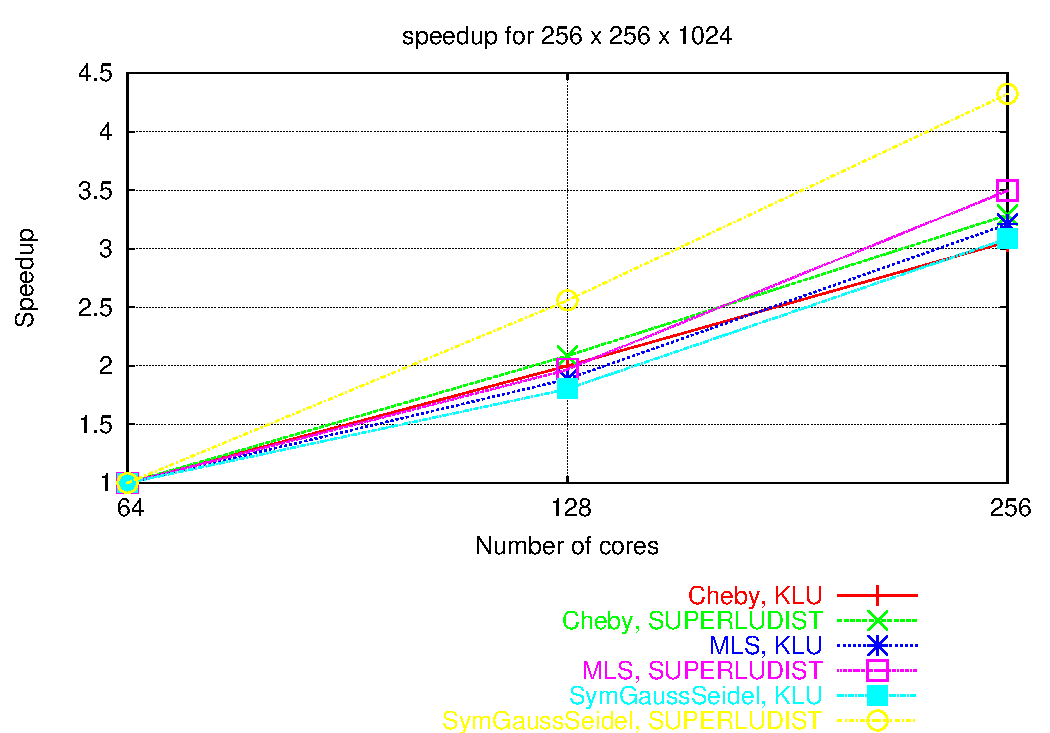
\includegraphics[width=0.85\textwidth]{plots/speedup_256_256_1024_3.pdf}
		\end{center}

	\end{frame}
	
	\begin{frame}
		\frametitle{Multigrid Parameters (2/2)}
		\framesubtitle{conduct measurements at CSCS}

		%graphs
		\begin{center}
			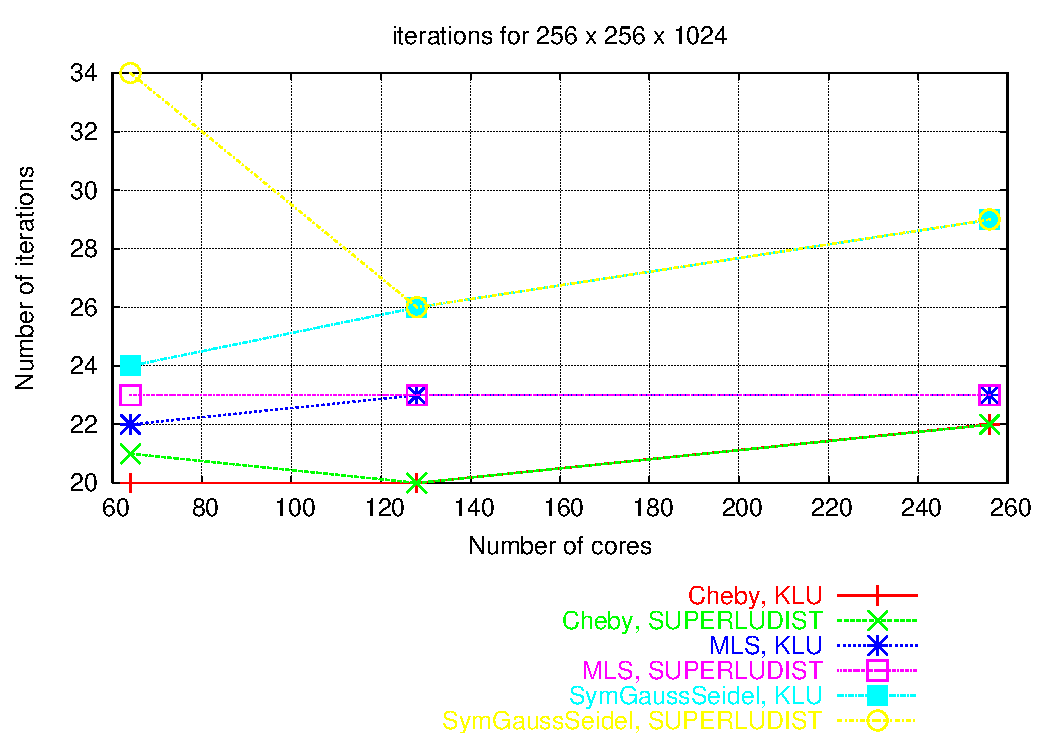
\includegraphics[width=0.85\textwidth]{plots/iterations_256_256_1024_3.pdf}
		\end{center}

	\end{frame}

	%\begin{frame}
	%	\frametitle{First Results}
	%	\framesubtitle{multigrid with "open" boundary condition}

	%	HOPEFULLY TILL NEXT WEEK

	%\end{frame}


    %CONTENT: sw-interpolation idea, ASK BENEDICT ABOUT geometry
    \section{Handling Boundary Conditions}
    	
	\begin{frame}
		\frametitle{Boundary Conditions: Nonrectangular Domains}
		\framesubtitle{Shortley-Weller approximation}
	
		\begin{columns}
		\begin{column}{4cm}	
			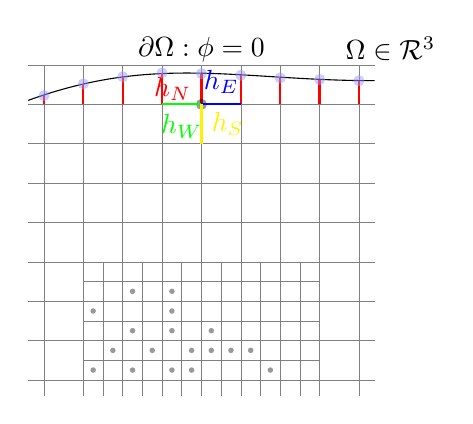
\begin{tikzpicture}[domain=-0.2:4.2,scale=1.0]
    \draw[very thin,color=gray,step=5mm] (-0.2,-0.2) grid (4.2,4);
    \draw[very thin,color=gray,step=2.5mm] (0.5,-0.2) grid (3.5,1.5);
    
    %\filldraw[fill=gray!20,fill opacity=0.8](2,2)--(2,3)--(3,3)--(3,2)--cycle;

    %curved boundart
    \draw (-0.2,3.55) to[out=20,in=180] node [sloped,below] {} (4.2,3.8);
    %\draw (-0.2,3.3) to[out=30,in=180] node [sloped,below] {$\Omega$} (4.2,3.8);
    
    %\coordinate [label=above:\C] (C) at (intersection of B and 1,0--1,1);
    %\fill[black,opacity=.5] C circle (2pt);
  
    %labels
    \node at (4.4,4.2) {$\Omega \in \mathcal{R}^3$};
    \node at (2,4.2) {$\partial \Omega: \phi = 0$};

    %interpolation lines
    \draw[thick,color=red] (0.0,3.5) to (0.0,3.61);
    \draw[thick,color=red] (0.5,3.5) to (0.5,3.76);
    \draw[thick,color=red] (1.0,3.5) to (1.0,3.85);
    \draw[thick,color=red] (1.5,3.5) to (1.5,3.90);
    \draw[thick,color=red] (2.0,3.5) to node[left] {$h_N$}(2.0,3.89);
    \draw[thick,color=red] (2.5,3.5) to (2.5,3.87);
    \draw[thick,color=red] (3.0,3.5) to (3.0,3.835);
    \draw[thick,color=red] (3.5,3.5) to (3.5,3.815);
    \draw[thick,color=red] (4.0,3.5) to (4.0,3.8);

    %on example interpol-point
    \fill[color=black,opacity=0.4] (2.0,3.5) circle (2pt);
    \draw[thick,color=green] (2.0,3.5) to node[below] {$h_W$} (1.5,3.5);
    \draw[thick,color=blue] (2.0,3.5) to node[above] {$h_E$} (2.5,3.5);
    \draw[thick,color=yellow] (2.0,3.5) to node[right] {$h_S$} (2.0,3.0);
    %\node at (2.2,3.7) {$h_{E}$};
    %\node at (1.7,3.7) {$h_{W}$};
    %\node at (2.2,3.2) {$h_{S}$};
    %\node at (2.2,3.2) {$h_{N}$};


    %short notice: dont use intersect
    \fill[blue!40,opacity=0.5] (0,3.61) circle (2pt);
    \fill[blue!40,opacity=0.5] (0.5,3.76) circle (2pt);
    \fill[blue!40,opacity=0.5] (1,3.85) circle (2pt);
    \fill[blue!40,opacity=0.5] (1.5,3.9) circle (2pt);
    \fill[blue!40,opacity=0.5] (2,3.89) circle (2pt);
    \fill[blue!40,opacity=0.5] (2.5,3.87) circle (2pt);
    \fill[blue!40,opacity=0.5] (3,3.835) circle (2pt);
    \fill[blue!40,opacity=0.5] (3.5,3.815) circle (2pt);
    \fill[blue!40,opacity=0.5] (4,3.8) circle (2pt);

    %particles
    \fill[black!40] (0.625,0.125) circle (1pt);
    \fill[black!40] (0.625,0.875) circle (1pt);
    
    \fill[black!40] (0.875,0.375) circle (1pt);

    \fill[black!40] (1.625,1.125) circle (1pt);
    
    \fill[black!40] (1.375,0.375) circle (1pt);

    \fill[black!40] (1.125,1.125) circle (1pt);
    \fill[black!40] (1.125,0.625) circle (1pt);
    \fill[black!40] (1.125,0.125) circle (1pt);
    
    \fill[black!40] (1.625,0.875) circle (1pt);
    \fill[black!40] (1.625,0.125) circle (1pt);
    \fill[black!40] (1.625,0.625) circle (1pt);

    \fill[black!40] (1.875,0.375) circle (1pt);
    \fill[black!40] (1.875,0.125) circle (1pt);
    
    \fill[black!40] (2.125,0.375) circle (1pt);
    \fill[black!40] (2.125,0.625) circle (1pt);

    \fill[black!40] (2.375,0.375) circle (1pt);

    \fill[black!40] (2.625,0.375) circle (1pt);
    
    \fill[black!40] (2.875,0.125) circle (1pt);

\end{tikzpicture}

		\end{column}
		\begin{column}{6.5cm}	
		\small{	
			\[
				2 \begin{bmatrix}
				& \frac{b}{h_N (h_N + h_S)} & \\
				\frac{a}{h_W (h_W + h_E)} & -\frac{a}{h_w h_E} -\frac{b}{h_S h_N} & \frac{a}{h_E (h_W + h_E)} \\
				& \frac{b}{h_S (h_N + h_S)} & \\
				\end{bmatrix}_h
			\] 
		}
		\end{column}
		\end{columns}

	\end{frame}

%	\begin{frame}
%		\frametitle{Boundary Conditions: Nonrectangular Domains (2/2)}
%		\framesubtitle{Shortley-Weller approximation}
%
%		For irregular interior grid points the five-point Shortley-Weller approxmiation is used:		
%
%		\[
%			2 \begin{bmatrix}
%			& \frac{b}{h_N (h_N + h_S)} & \\
%			\frac{a}{h_W (h_W + h_E)} & -\frac{a}{h_w h_E} -\frac{b}{h_S h_N} & \frac{a}{h_E (h_W + h_E)} \\
%			& \frac{b}{h_S (h_N + h_S)} & \\
%			\end{bmatrix}_h
%		\]
%
%		\vspace{0.8cm}
%
%		HW restriction and linear interpolation should result in decent convergence (to be examined)
%
%	\end{frame}
	
	\begin{frame}
		\frametitle{Geometry of Boundary Conditions}
		\framesubtitle{importing BC geometry}

		\begin{center}
			\tikzstyle{format} = [draw, thin, fill=blue!20]
\tikzstyle{pblock} = [rectangle, draw, fill=blue!20, text width=6em, text centered, rounded corners, minimum height=0.4em]
\tikzstyle{mblock} = [rectangle, draw, fill=green!20, text width=6em, text centered, rounded corners, minimum height=0.4em]
\tikzstyle{bblock} = [rectangle, draw, fill=gray!20, text width=6em, text centered, rounded corners, minimum height=0.4em]
\tikzstyle{prblock} = [rectangle, draw, fill=red!20, text width=6em, text centered, rounded corners, minimum height=0.4em]
\tikzstyle{rblock} = [rectangle, draw, fill=olive!20, text width=6em, text centered, rounded corners, minimum height=0.4em]
%\tikzstyle{block} = [rectangle, draw, fill=blue!20, text centered, rounded corners]
\tikzstyle{decision} = [diamond, draw, fill=blue!20, text width=4.5em, text badly centered, node distance=3cm, inner sep=0pt]
\tikzstyle{medium} = [ellipse, draw, thin, fill=green!20, minimum height=2.5em]
\tikzstyle{cloud} = [draw, ellipse,fill=red!20, node distance=3cm, minimum height=2em]
\tikzstyle{line} = [draw, -latex']
\tikzstyle{emptyblock} = [rectangle]


\begin{tikzpicture}[scale=0.8,transform shape,node distance=3cm]%[node distance = 3cm, scale=0.5]
    % Place nodes
    \node [pblock] (STEP) {
		     STEP file};
    \node [bblock, right of=STEP] (BOGUI) {
		     heronion};
    \node [mblock, right of=BOGUI] (surfmesh) {
		     surface mesh};
    \node [mblock, below of=surfmesh] (add) {
		     mesh, ...};
    \node [pblock, right of=surfmesh] (H5FED) {
		     H5FED};
    \node [pblock, above of=H5FED] (H5Part) {
		     H5Part};

    \node [pblock, below of=H5FED] (VTK) {
    		     VTK};
    \node [bblock, right of=H5FED] (OPAL) {
    		     OPAL};
		  
    % Draw edges
    \path [line] (STEP) -> (BOGUI);
    \path [line] (BOGUI) -> (surfmesh);
    \path [line,style=dashed, ->] (BOGUI) edge [out=-90, in=90] (add);
    \path [line] (surfmesh) -> (H5FED);
    \path [line,style=dashed, ->] (surfmesh) edge [out=-90, in=90] (VTK);
    %\path [->] (fifth) edge [out=-90, in=90] (distmesh);
    \path [->] (H5FED) edge (OPAL);
    \path [line,style=dashed, ->] (H5FED) edge [out=90, in=180] node[right] {part of} (H5Part);
    \path [<->] (H5Part) edge [out=0, in=90] (OPAL);
    

\end{tikzpicture}

%\begin{tikzpicture}[overlay]
%	\path[->]<1-> (third) (fifth);
%	\path[->,red!40,thick]<2-> (second) edge [bend right] (fifth);
%\end{tikzpicture}

		\end{center}

		\small{in collaboration with B. Oswald and A. Gsell (AIT)}

	\end{frame}

    \section{Further Work}

    	\begin{frame}
		\frametitle{Further Work}

		After having completely tested and implemented the electrostatic solver with the described Multigrid method and BC, the next tasks are:

		\vspace{0.5cm}

		\begin{itemize}
			\item reuse information we have about the stencil to accelerate convergence
			\item implement own aggregation schemes (save graph)
			\item investigate and implement adaptive mesh refinement algorithms (P. Colella et al.)
		\end{itemize}

	\end{frame}
    	
	\begin{frame}
		\frametitle{Timetable}

	                \begin{center}
                        \rowcolors{1}{blue!20}{blue!5}
                        \begin{tabular}{|c|c|}
                        \hline
                        Task & approx. Completion \\
                        \hline
                        integrating ML in OPAL & mid - end of April \\
                        simple geometry Shortley-Weller BC (pipe) & end of May \\
                        complicated geometry (STEP) & mid June \\
			various improvements and speedups & end July \\
			end of master thesis & 17. August \\
                        \hline
                        \end{tabular}
	                \end{center}
	

	\end{frame}

     \section{Summary}

     	\begin{frame}
		\frametitle{Summary}

		%TODO: stress goals/impr
		\textbf{Improved Space Charge Solver:} \\
		solution of previous timesteps can be used as initial guess

		\begin{itemize}
			\item \color{green}{is discretized with finite differences}
			\item \color{green}{is solved with a multi-level preconditioned CG}
			\item \color{green}{anisotropies can be handled}
			\item \color{green}{uses smoothed aggregation}
			\item \alert{fully integrated into OPAL}
		\end{itemize}

		\vspace{0.4cm}

		\textbf{Improved Boundary Conditions:} \\
		uses exact geometry information of the beam pipe

		\begin{itemize}
			\item \alert{Shortly-Weller interpolation}
			\item \alert{STEP files can be used (heronion)}
		\end{itemize}

	\end{frame}
 
	%\begin{frame}
	%  	\frametitle{Questions?}
	%	\begin{center}
	%		\LARGE{Questions?}
	%	\end{center}
	%\end{frame}
	
	\begin{frame}
	  	\frametitle{Backup}
		\begin{center}
			\LARGE{Backup}
		\end{center}
	\end{frame}
	
  \begin{frame}
		\frametitle{Grid Operators}
		\framesubtitle{AMG: smoothed aggregation}

		%TODO: finish

		Operate on directly on (linear sparse) algebraic equations:

		\[
			\sum_j a_{ij}^h x_j^h = b_i^h
		\]

		\begin{itemize}
			\item replace "grid" with "variables"
			%\item AMG fixes smoother and adjusts coarsening (GMG inverse)
			\item coarse level equations are generated without the use of any geometry
			\item no coarse level grids have to be generated or stored
			\item good preconditioner: works on all error components (in contrast to level-one precond)
		\end{itemize}

		\vspace{0.2cm}
		SA restrict operator:

		\[
			I_H^h = (I_h - \omega D_h^{-1} A_h^f) \hat{I}_H^h
		\]

		%generate operator dependet interpolation and Galerkin operator can be derived directly from the underlying matrices, without any reference to the actual grids.
	
	\end{frame}

%	\appendix
%	\begin{frame}
%	  \frametitle<presentation>{References}
%	  \begin{thebibliography}{10}
%	  \beamertemplatearticlebibitems
%	
%	  \bibitem{BAISU2005}
%	    Z.\ Bai. \scriptsize{AND} \normalsize{Y.\ Su.}
%	    \newblock {\em SOAR: A Second-Order Arnoldi Method for the Solution of the Quadratic Eigenvalue Problem}.
%	    \newblock SIAM J. Matrix Anal. Appl., 2005.
%
%	  \bibitem{PRESVAR}
%	    \textbf{L.\ Lee.}, L.\ Ge., Z.\ Li., C.\ Ng., K.\ Ko., B.\ Liao., Z.\ Bai., D.\ Gao., W.\ Gao., C.\ Yang., P.\ Husbands., E.G.\ Ng.
%	    \newblock{\em Solving Nonlinear Eigenproblems in Acclerator Cavity Design}.
%	    \newblock SIAM Annual Meeting, MS 44 and MS 56: Nonlinear Eigenvalue Problems, 2005
%	    
%	  \end{thebibliography}
%	\end{frame}

\end{document}
